
\documentclass[12pt]{article}
%\usepackage[finnish]{babel}
\usepackage[T1]{fontenc}
\usepackage[utf8]{inputenc}
\usepackage{amssymb}
\usepackage{amsmath}
\usepackage{graphicx}
\usepackage{hyperref}
\newcommand{\pat}{\partial}
\newcommand{\be}{\begin{equation}}
\newcommand{\ee}{\end{equation}}
\newcommand{\bea}{\begin{eqnarray}}
\newcommand{\eea}{\end{eqnarray}}
\newcommand{\abf}{{\bf a}}
\newcommand{\Zcal}{{\cal Z}_{12}}
\newcommand{\zcal}{z_{12}}
\newcommand{\Acal}{{\cal A}}
\newcommand{\Fcal}{{\cal F}}
\newcommand{\Ucal}{{\cal U}}
\newcommand{\Vcal}{{\cal V}}
\newcommand{\Ocal}{{\cal O}}
\newcommand{\Rcal}{{\cal R}}
\newcommand{\Scal}{{\cal S}}
\newcommand{\Lcal}{{\cal L}}
\newcommand{\Hcal}{{\cal H}}
\newcommand{\hsf}{{\sf h}}
\newcommand{\half}{\frac{1}{2}}
\newcommand{\Xbar}{\bar{X}}
\newcommand{\xibar}{\bar{\xi }}
\newcommand{\barh}{\bar{h}}
\newcommand{\Ubar}{\bar{\cal U}}
\newcommand{\Vbar}{\bar{\cal V}}
\newcommand{\Fbar}{\bar{F}}
\newcommand{\zbar}{\bar{z}}
\newcommand{\wbar}{\bar{w}}
\newcommand{\zbarhat}{\hat{\bar{z}}}
\newcommand{\wbarhat}{\hat{\bar{w}}}
\newcommand{\wbartilde}{\tilde{\bar{w}}}
\newcommand{\barone}{\bar{1}}
\newcommand{\bartwo}{\bar{2}}
\newcommand{\nbyn}{N \times N}
\newcommand{\repres}{\leftrightarrow}
\newcommand{\Tr}{{\rm Tr}}
\newcommand{\tr}{{\rm tr}}
\newcommand{\ninfty}{N \rightarrow \infty}
\newcommand{\unitk}{{\bf 1}_k}
\newcommand{\unitm}{{\bf 1}}
\newcommand{\zerom}{{\bf 0}}
\newcommand{\unittwo}{{\bf 1}_2}
\newcommand{\holo}{{\cal U}}
\newcommand{\bra}{\langle}
\newcommand{\ket}{\rangle}
\newcommand{\muhat}{\hat{\mu}}
\newcommand{\nuhat}{\hat{\nu}}
\newcommand{\rhat}{\hat{r}}
\newcommand{\phat}{\hat{\phi}}
\newcommand{\that}{\hat{t}}
\newcommand{\shat}{\hat{s}}
\newcommand{\zhat}{\hat{z}}
\newcommand{\what}{\hat{w}}
\newcommand{\sgamma}{\sqrt{\gamma}}
\newcommand{\bfE}{{\bf E}}
\newcommand{\bfB}{{\bf B}}
\newcommand{\bfM}{{\bf M}}
\newcommand{\cl} {\cal l}
\newcommand{\ctilde}{\tilde{\chi}}
\newcommand{\ttilde}{\tilde{t}}
\newcommand{\ptilde}{\tilde{\phi}}
\newcommand{\utilde}{\tilde{u}}
\newcommand{\vtilde}{\tilde{v}}
\newcommand{\wtilde}{\tilde{w}}
\newcommand{\ztilde}{\tilde{z}}


\hoffset 0.5cm
\voffset -0.4cm
\evensidemargin -0.2in
\oddsidemargin -0.2in
\topmargin -0.2in
\textwidth 6.3in
\textheight 8.4in

\begin{document}

\normalsize

\baselineskip 14pt

\begin{center}
{\Large {\bf FYMM/MMP IIIa 2020 \ \ \  Solutions to Problem Set 6}}
Jake Muff
10/11/20
\end{center}

\bigskip

\noindent



\begin{enumerate}
\item {\bf Mattress flipping.}\\
In this question we have 4 different operations:
\begin{enumerate}
    \item I $\rightarrow$ do nothing, the identity operation 
    \item R $\rightarrow$ flip 180 degrees along the long side 
    \item P $\rightarrow$ flip 180 degrees along the short side 
    \item Y $\rightarrow$ rotation of 180 degrees around the center 
\end{enumerate}
%figure 1
\begin{figure}[h]
    \centering
    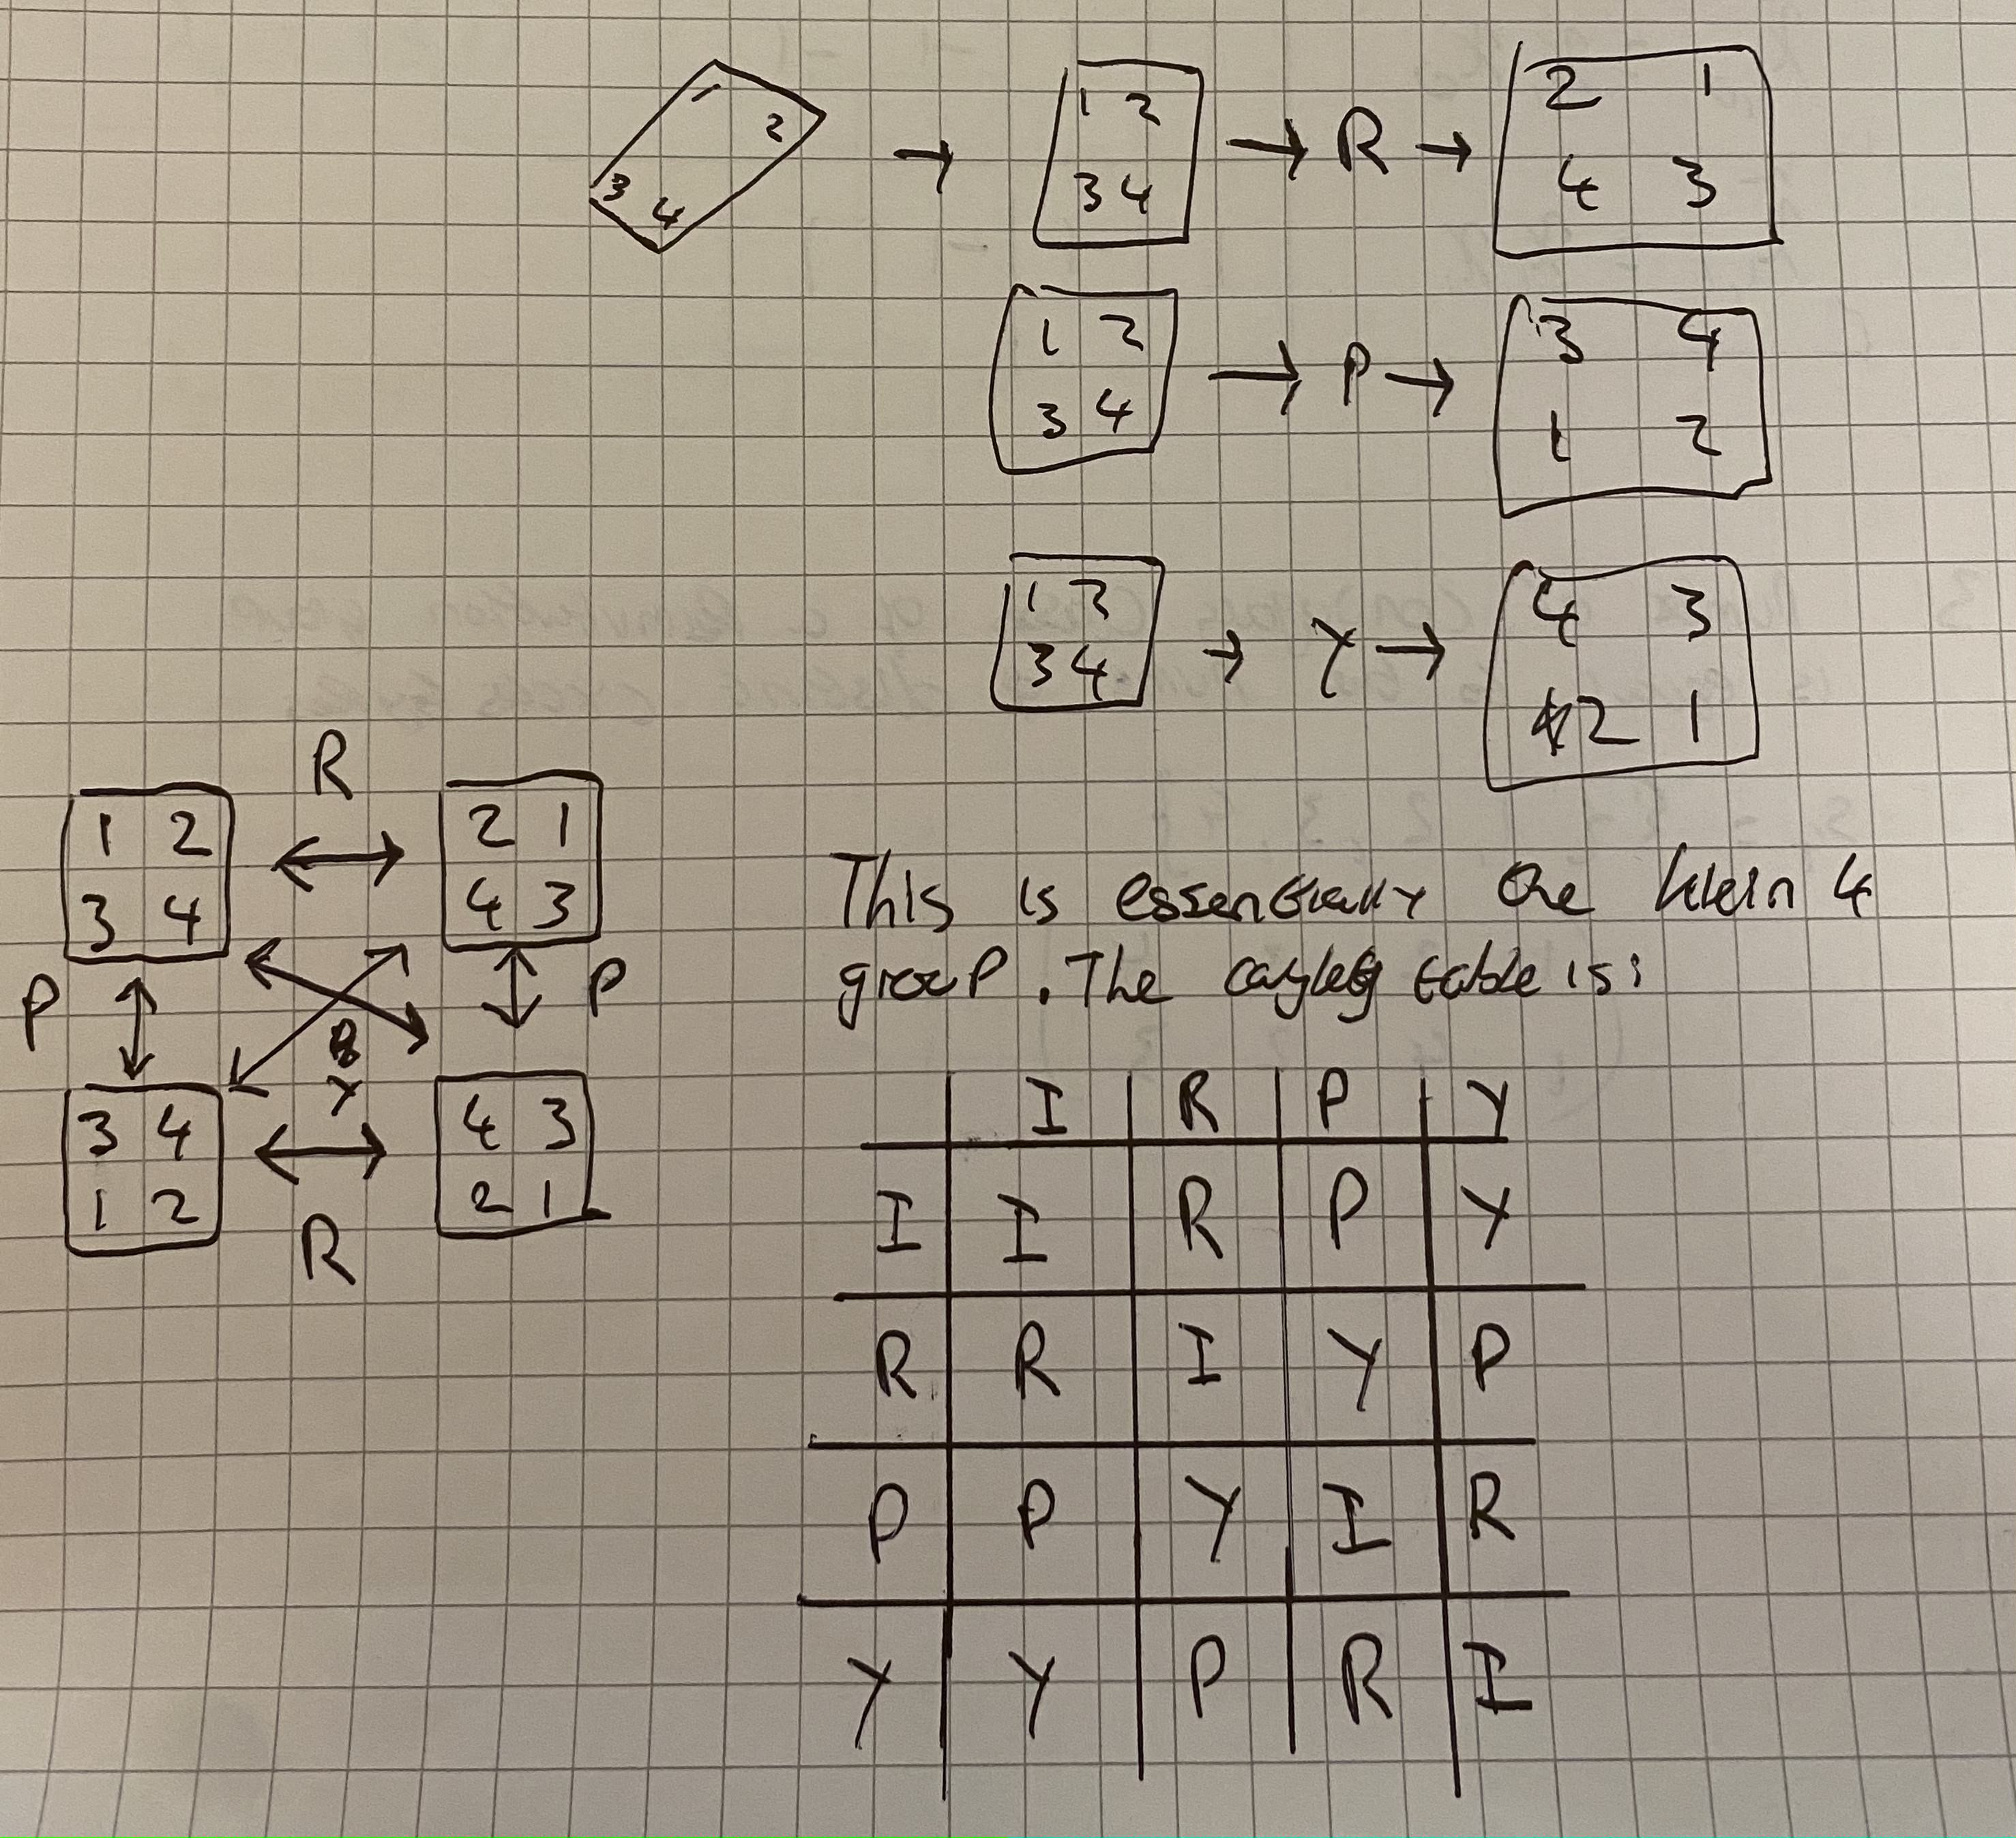
\includegraphics[width=10cm]{q1.jpg}
    \caption{Picture of Mattress flipping diagrams. Don't know why they have rendered badly. Will attach also.}
    \end{figure}
%figure 2

This is essentially the klein 4 group 
%table 1
\begin{table}[h]
    \centering
    \begin{tabular}{lllll}
                           & I                      & R                      & P                      & Y                      \\ \cline{2-5} 
    \multicolumn{1}{l|}{I} & \multicolumn{1}{l|}{I} & \multicolumn{1}{l|}{R} & \multicolumn{1}{l|}{P} & \multicolumn{1}{l|}{Y} \\ \cline{2-5} 
    \multicolumn{1}{l|}{R} & \multicolumn{1}{l|}{R} & \multicolumn{1}{l|}{I} & \multicolumn{1}{l|}{Y} & \multicolumn{1}{l|}{P} \\ \cline{2-5} 
    \multicolumn{1}{l|}{P} & \multicolumn{1}{l|}{P} & \multicolumn{1}{l|}{Y} & \multicolumn{1}{l|}{I} & \multicolumn{1}{l|}{R} \\ \cline{2-5} 
    \multicolumn{1}{l|}{Y} & \multicolumn{1}{l|}{Y} & \multicolumn{1}{l|}{P} & \multicolumn{1}{l|}{R} & \multicolumn{1}{l|}{I} \\ \cline{2-5} 
    \end{tabular}
    \caption{Cayley table for operations in the mattress flipping}
    \end{table}

This is the klein four group also known as the viergruppe $\mathbb{Z}_2 \times \mathbb{Z}_2$ group with a matching cayley table

\item Construct the character table of $\mathbb{Z}_2\times \mathbb{Z}_2$.
\\
\begin{table}[h]
    \centering
    \begin{tabular}{lllll}
                                                           & (0,0)                  & (0,1)                   & (1,0)                   & (1,1)                   \\ \hline
    \multicolumn{1}{|l|}{$\chi_{0,1}^{~} = \chi_0 \chi_0$} & \multicolumn{1}{l|}{1} & \multicolumn{1}{l|}{1}  & \multicolumn{1}{l|}{1}  & \multicolumn{1}{l|}{1}  \\ \hline
    \multicolumn{1}{|l|}{$\chi_{0,1} = \chi_0 \chi_1$}     & \multicolumn{1}{l|}{1} & \multicolumn{1}{l|}{-1} & \multicolumn{1}{l|}{1}  & \multicolumn{1}{l|}{-1} \\ \hline
    \multicolumn{1}{|l|}{$\chi_{1,0} = \chi_1 \chi_0$}     & \multicolumn{1}{l|}{1} & \multicolumn{1}{l|}{1}  & \multicolumn{1}{l|}{-1} & \multicolumn{1}{l|}{-1} \\ \hline
    \multicolumn{1}{|l|}{$\chi_{1,1} = \chi_1 \chi_1$}     & \multicolumn{1}{l|}{1} & \multicolumn{1}{l|}{-1} & \multicolumn{1}{l|}{-1} & \multicolumn{1}{l|}{1}  \\ \hline
    \end{tabular}
    \caption{Character table for $\mathbb{Z}_2 \times \mathbb{Z}_2$}
    \label{tab:my-table}
    \end{table}

\item Proving that the number of conjugacy classes of a permutation group is equal to the number of disjoint cycle types. 
$$ S_4 = \{ 1,2,3,4\} $$
$$  \left( \begin{array}{cccccc} 1 & 2 & 3 & 4 \\ 1 & 4 & 2 & 3 \end{array}\right) $$
The $S_4$ has cycle types of 
$$ (12), (13), (14), (23), (24), (34) \rightarrow 2-cycles $$
$$ (12)(34), (13)(24), (14)(23) \rightarrow Products of 2-cycles$$
$$ (123), (124), (132), (134), (142), (143), (234), (243) \rightarrow 3-cycles $$
$$ (1234), (1234), (1324), (1342), (1423), (1432) \rightarrow 4-cycles $$

Along the the cycle type $()$ i.e the empty cycles which sometimes denoted $e$, we have 5 cycle types. The character table for $S_4$ shows:
\begin{table}[h]
    \centering
    \begin{tabular}{lccccc}
                                                                      & \multicolumn{1}{l}{()} & \multicolumn{1}{l}{(1,2)(3,4)} & \multicolumn{1}{l}{(1,2)} & \multicolumn{1}{l}{(1,2,3,4)} & \multicolumn{1}{l}{(1,23)} \\ \hline
    \multicolumn{1}{|l|}{Trivial representation}                      & \multicolumn{1}{c|}{1} & \multicolumn{1}{c|}{1}         & \multicolumn{1}{c|}{1}    & \multicolumn{1}{c|}{1}        & \multicolumn{1}{c|}{1}     \\ \hline
    \multicolumn{1}{|l|}{Sign representation}                         & \multicolumn{1}{c|}{1} & \multicolumn{1}{c|}{1}         & \multicolumn{1}{c|}{-1}   & \multicolumn{1}{c|}{-1}       & \multicolumn{1}{c|}{1}     \\ \hline
    \multicolumn{1}{|l|}{Irreducible representation}                  & \multicolumn{1}{c|}{2} & \multicolumn{1}{c|}{2}         & \multicolumn{1}{c|}{0}    & \multicolumn{1}{c|}{0}        & \multicolumn{1}{c|}{-1}    \\ \hline
    \multicolumn{1}{|l|}{Standard representation}                     & \multicolumn{1}{c|}{3} & \multicolumn{1}{c|}{-1}        & \multicolumn{1}{c|}{1}    & \multicolumn{1}{c|}{-1}       & \multicolumn{1}{c|}{0}     \\ \hline
    \multicolumn{1}{|l|}{Product of standard and sign representation} & \multicolumn{1}{c|}{3} & \multicolumn{1}{c|}{-1}        & \multicolumn{1}{c|}{-1}   & \multicolumn{1}{c|}{1}        & \multicolumn{1}{c|}{0}     \\ \hline
    \end{tabular}
    \caption{Character table for $S_4$}
    \label{table 3}
    \end{table}
Which has 5 conjugacy classes. This shows that for $S_4$ the number of classes is equal to the number of cycle types. 
\begin{figure}[h]
    \centering
    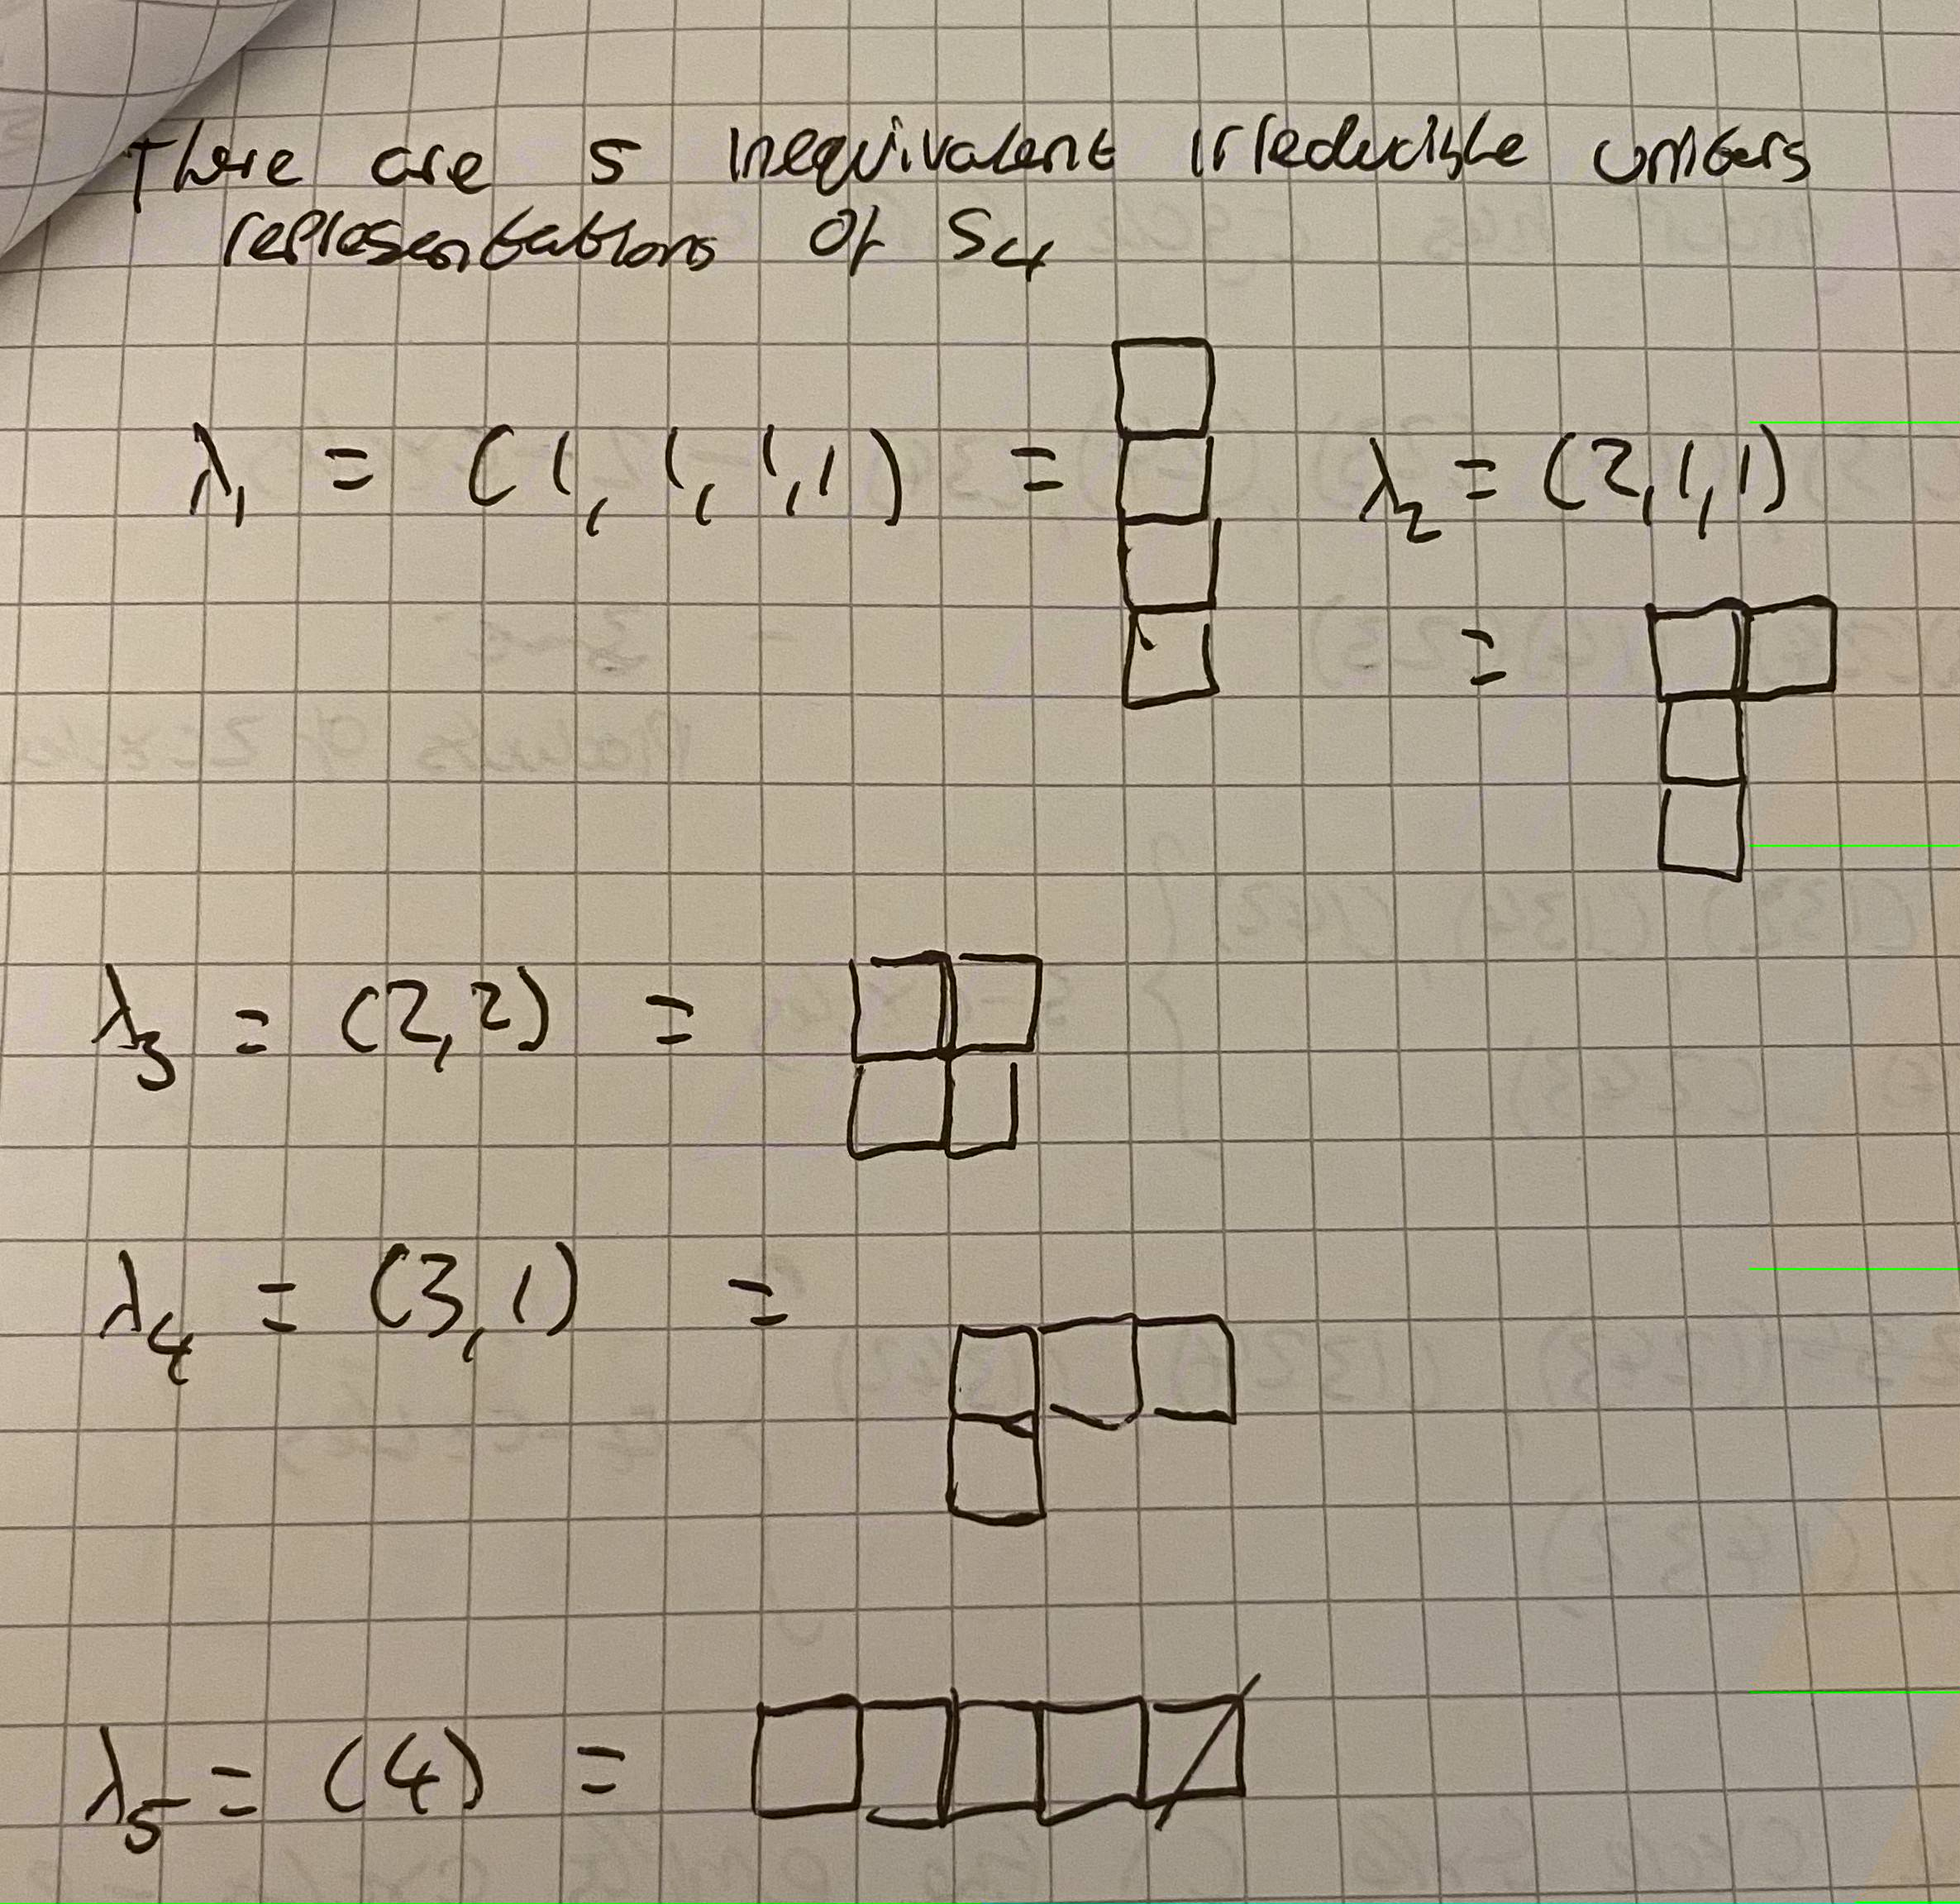
\includegraphics[width=10cm]{youngstable.jpg}
    \caption{Young diagrams for $S_4$ also showing 5 inequivalent irreducible unitary representations}
    \end{figure}

\item Given a vector space $V$, prove that every $\omega \in (V^*)^*$ can be uniquely associated with a vector $\vec{v}\in V$ such that $\omega (f)= \bra f , \vec{v}\ket$.
We know that $\omega \in (V^*)^*$ is a dual of a dual such that $\omega: V^* \rightarrow \mathbb{C}$. A vector can be written as 
$$ \vec{v} = v^j \vec{e}_j $$
The dual basis is 
$$ e^{*j} (\vec{e}_j) = \delta_j^i \rightarrow \ dim V = dim V^* = n$$ 
Let $f$ be a linear function with $v \in \mathbb{C}$ 
$$ f(\vec{v}) = f_i e^{*i} (v^j \vec{e}_j) = f_i v^j e^{*i} (\vec{e}_j) $$
$$ = f_i v^i \delta^i_j = f_i v^i = \langle f, \vec{v} \rangle $$
So for $\omega (f)$ 
$$ \omega(f) = v_i e^{**i}(f) = v_i e^{**i} (f^j \vec{e}_j) = v_i f^j e^{**i} (\vec{e}^*_j) $$
$$  = v_i f^j \delta^i_j = v_i f^i = f_i v^i = \langle f, \vec{v} \rangle $$



\item Let the (1,0)-tensor $R$
have the components
$$
R^1=a \ ; R^2 = a^2 \ ; R^3 = a^4 
$$
and the (0,1)-tensor $S$
have the components
$$
S_1=-b \ ; S_2 = c \ ; S_3 =- d \ . 
$$
Calculate all the components $T^\mu_\nu$ of the (1,1)-tensor $T=R\otimes S$.
\\
$$ T_1^1 = R^1 S_1 = -ab \ \ T^2_1 = R^2 S_1 = -a^2 b $$
$$ T_2^1 = R^1 S_2 = ac \ \ T^2_2 = R^2 S_2 = a^2 c $$
$$ T_3^1 = R^1 S_3 = -ad \ \ T_3^2 = R^2 S_3 = -a^2 d $$
$$ T_1^3 = R^3 S_1 = -a^4 b \ \ T_2^3 = R^3 S_2 = a^4 c $$
$$ T_3^3 = R^3 S_3 = -a^4 d $$

\end{enumerate}
\end{document}
